\documentclass[a4paper]{article}
\usepackage[utf8]{inputenc}
\usepackage[italian]{babel}
\usepackage[T1]{fontenc}
\usepackage{amsmath,amssymb,amsthm}
\usepackage{enumerate}
\usepackage{epigraph}
\usepackage{fontspec}
\usepackage{graphicx}
\usepackage{hyperref}

\graphicspath{ {./images/} }

\title{
  {
    \fontspec{Symbola}
    \symbol{"1F17C}
    \symbol{"1F435}
    \symbol{"1F17D}
    \symbol{"1F17A}
  }ey \\
  \small Relazione del progetto per l'insegnamento di Algoritmi e strutture di
  dati
}
\author{
  Gaia Clerici (\#971338),
  Stefano Volpe (\#969766)
}

\date{
	Universit\`a di Bologna \\
  \today
}

\begin{document}

\maketitle

\begin{figure}[h]
  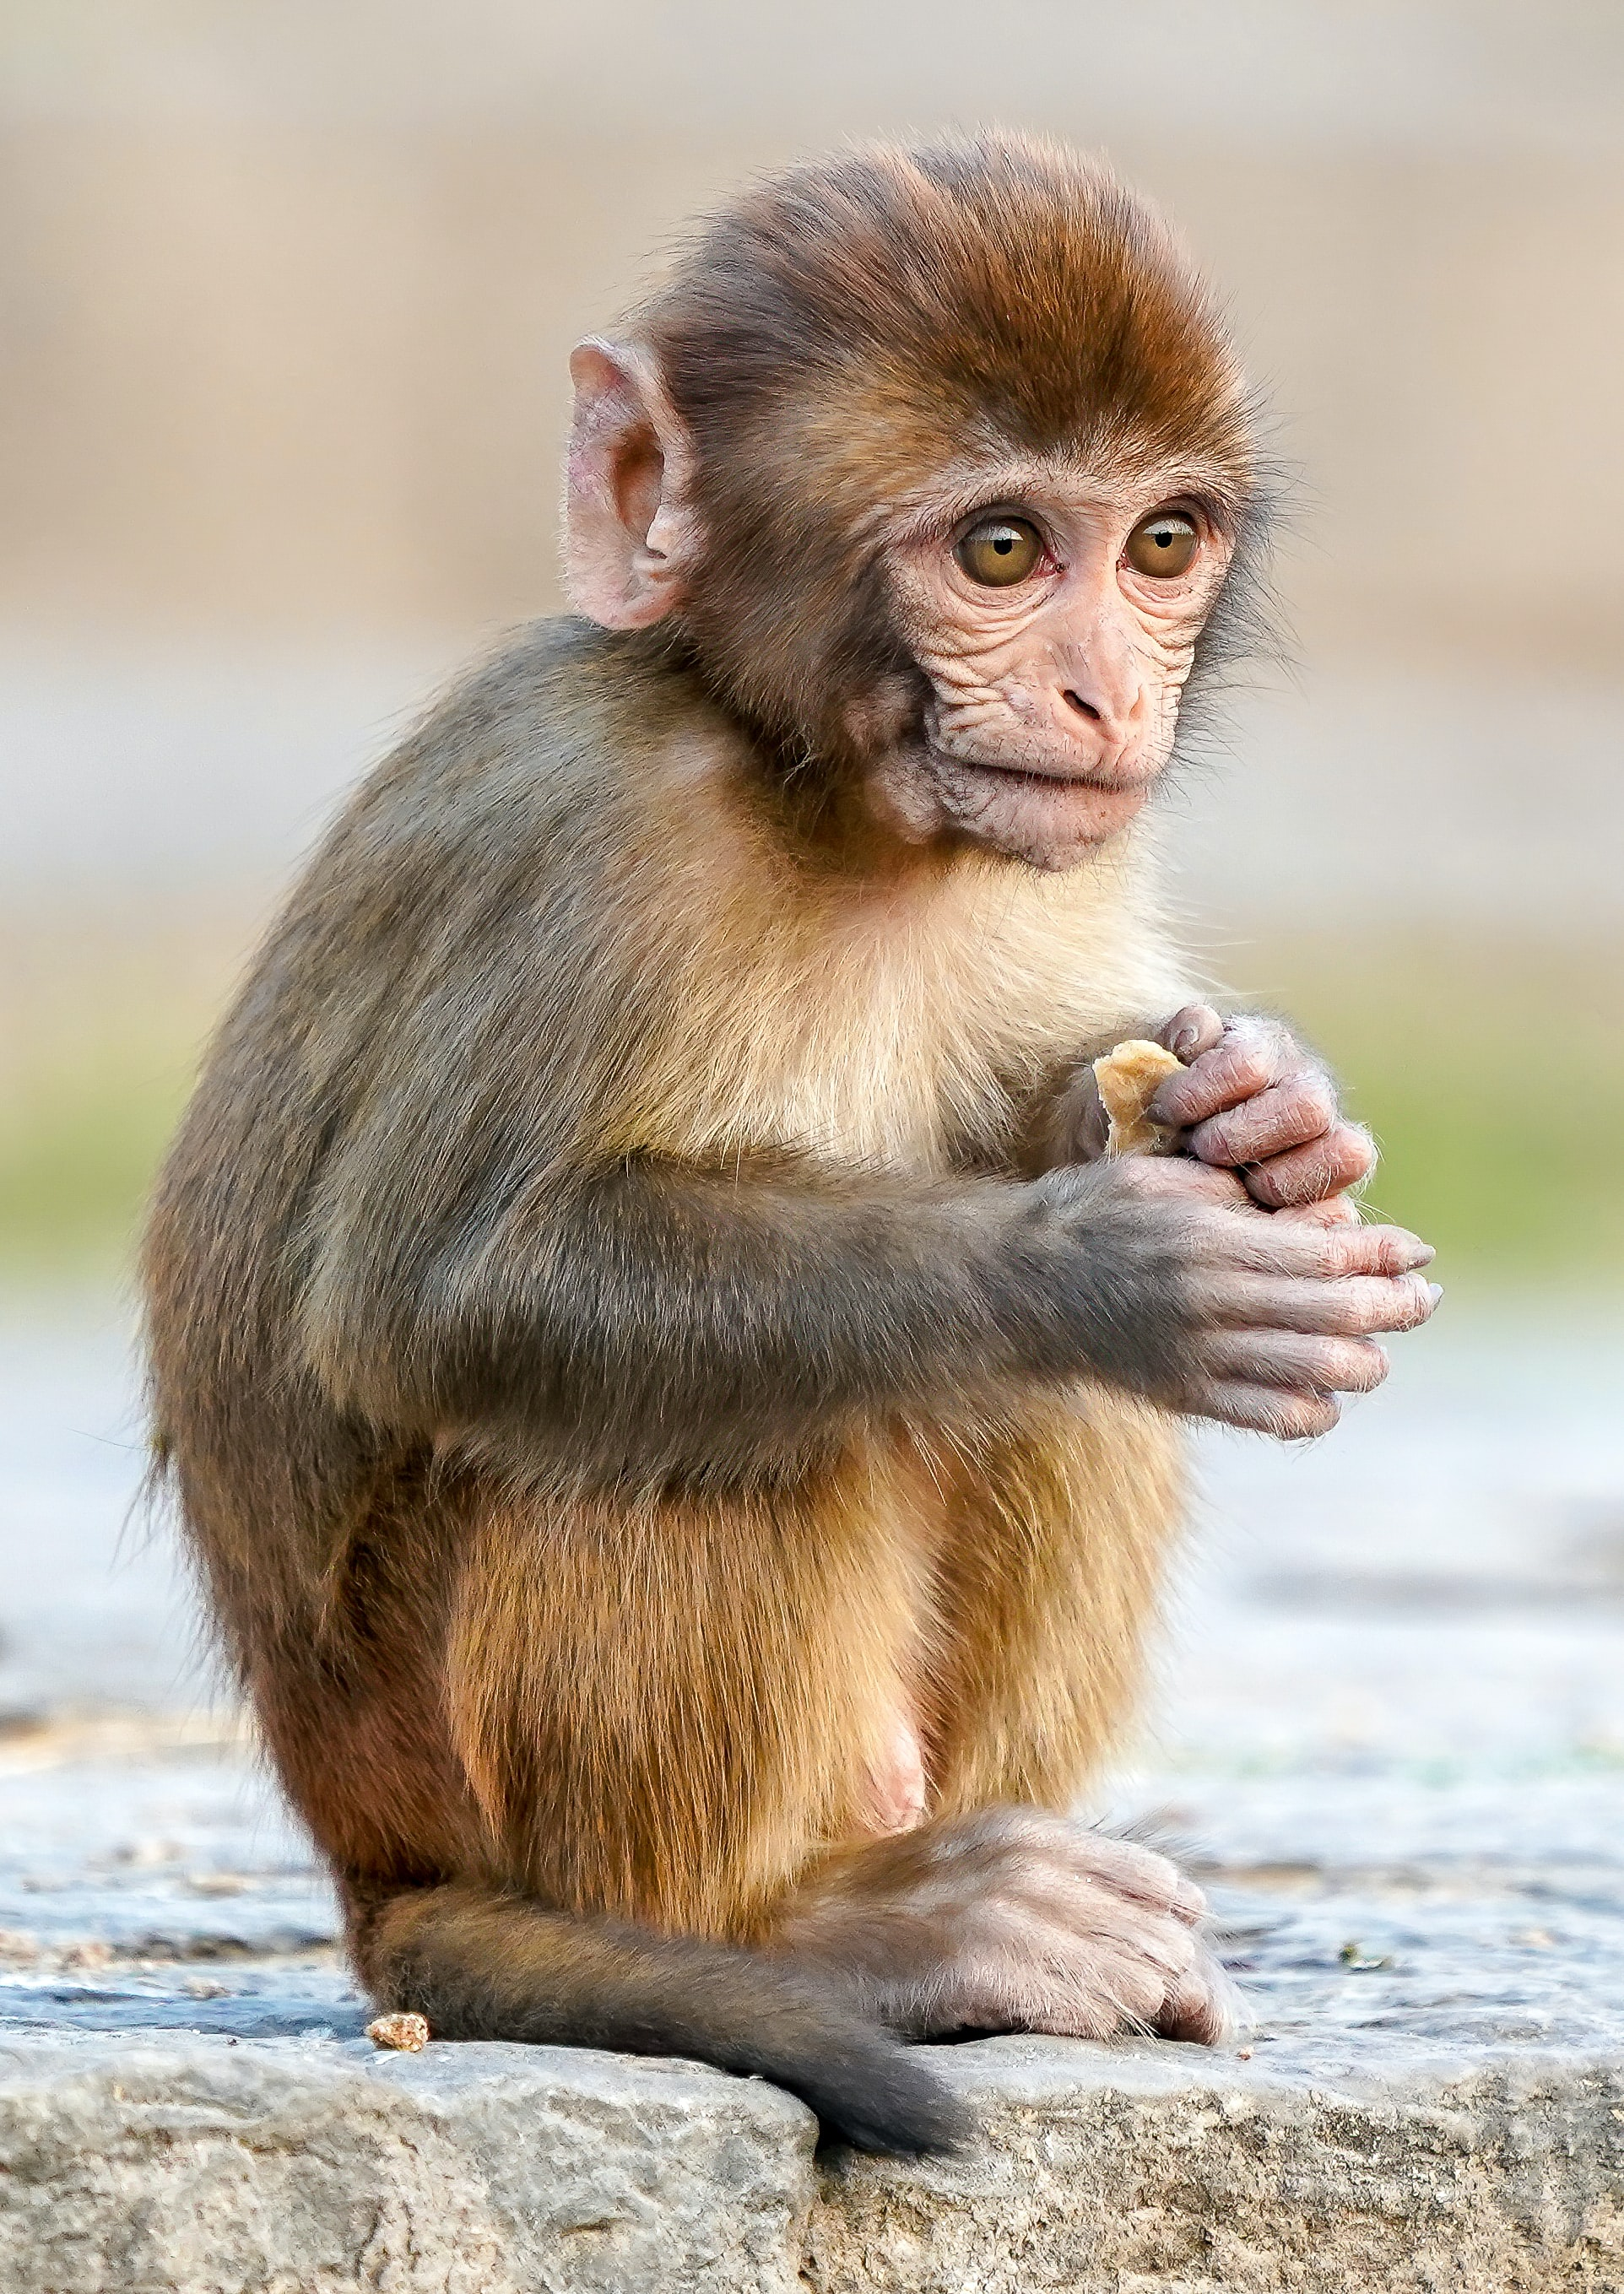
\includegraphics[width=0.75\textwidth]{monkey}
  \centering
  \caption{\href{https://unsplash.com/photos/daC7ji1EMHM}{una scimmia
  (foto di Bob Brewer)}}
\end{figure}

\pagebreak

\epigraph{Be a good little monkey.}{\textit{The Man with The Yellow Hat}}

\section{Analisi del problema}

\section{Scelte progettuali}

\section{Bibliografia}

\end{document}
